\documentclass{manual}

\title{Getting Started with CoaSim}
\subtitle{An introduction to the simulator CoaSim}
\authors{Thomas Mailund}
\contact{mailund@birc.dk}
\company{Bioinformatics ApS}
\toolversion{CoaSim v3.1}

\usepackage{wrapfig}

\begin{document}

\section{About CoaSim}

CoaSim is a tool for simulating the coalescent process with
recombination and geneconversion, under either constant population
size or exponential population growth.  It effectively constructs the
ancestral recombination graph for a given number of chromosomes and
uses this to simulate samples of SNP and micro-satellite haplotypes or
genotypes.

\subsection{Installing CoaSim}

CoaSim comes in two flavours: A graphical user interface version for
easy use by novice users, and a guile-scheme based version for
efficient scripting.  Both versions are distributed as RPM files or as
source code.  For most users, we recommend installing from the RPM
files, since building the tool from source requires setting up the
right build environment and having access to the needed development
tools.  If you are not familiar with UNIX C++ development, using the
Automake suite of tools, we do not recommend that you try building
from source.  If you are not familiar with Qt development, we do not
recommend that you try to build the GUI version from source.

\paragraph{Installing the RPM Files.}

The RPM files (\verb?coasim-gui-x.y.z-r.i386.rpm? and
\verb?coasim-guile-x.y.z-r.i386.rpm?, respectively) contains binary
versions of the program, compiled to an Intel x86 Linux platform.  To
install the graphical user interface version from the RPM package, run
\begin{code}
> rpm -Uvh coasim-gui-x.y.z-r.i386.rpm
\end{code}
where \texttt{x.y.z-r} is the version number of Coasim.  To install
the scheme version, run
\begin{code}
> rpm -Uvh coasim-guile-x.y.z-r.i386.rpm
\end{code}
Since the RPM files installs in the directory \verb?/usr/local/?,
installing the RPM package requires root access.

\paragraph{Installing from the Source Files.}

The source code is distributed in three tar-files:
\begin{itemize}
\item \verb?coasim-core-x.y.z.tar.gz?,
\item \verb?coasim-guile-x.y.z.tar.gz?, and
\item \verb?coasim-gui-x.y.z.tar.gz?.
\end{itemize}

The core files are needed for both the guile-scheme version while the
two remaining tar-balls are for the scheme and GUI version,
respectively.  To build the source files, first untar the core module
and place it in a directory called Core:

\begin{code}
> tar zxf coasim-core-x.y.z.tar.gz
> mv coasim-core-x.y.z Core
> cd Core
> ./configure
> make
\end{code}

To build the guile version, untar the source files next to the Core
module, configure and build:

\begin{code}
> cd ..
> tar zxf coasim-guile-x.y.z.tar.gz
> cd coasim-guile-x.y.z
> ./configure
> make
> make install
\end{code}

To build the GUI version, untar the source files next to the Core
module, install the designer plugins used, then qmake and build:

\begin{code}
> cd ..
> tar zxf coasim-gui-x.y.z.tar.gz
> cd coasim-gui-x.y.z/designer_plugins
> qmake
> make install
> cd ..
> qmake
> make
> make install
\end{code}

If you do not have write access to \verb?QTDIR/plugins?, you will need
to install the plugins locally, e.g. use qtconfig to add
\verb?$(HOME)/.qt/plugins? to the plugin path and do:

\begin{code}
> cd ..
> tar zxf coasim-gui-x.y.z.tar.gz
> cd coasim-gui-x.y.z/designer_plugins
> qmake
> INSTALL_ROOT=~/.qt make install
> cd ..
> qmake
> make
> make install
\end{code}


\subsection{Running CoaSim}

Installing the graphical user installing version should, on GNOME or
KDE desktops, add an icon in the start menu for running CoaSim.  If
this is not the case, the tool can be started on the command-line with
the command
\begin{code}
> coasim_gui
\end{code}

The scheme based version is started from the command-line; the
parameters for the simulation or simulations to be run is described in
one or more configuration scripts, which are written in the Scheme
programming language, see the \textit{CoaSim Scheme} manual for
documentation.  Starting CoaSim with the configuration script
\verb?simulation.scm?  is done as:
\begin{code}
> coasim_guile simulation.scm
\end{code}
Run \verb?coasim_guile --help? to get a complete list of command-line
options accepted by CoaSim.


\section{Using CoaSim}

Running CoaSim will in most cases consist of three steps: Set up the
simulation parameters, including the markers (type of marker, mutation
rates and similar), demographic parameters, rates for recombination,
etc.; running the simulation obtaining and ARG; and extracting the
needed information from the ARG (\emph{Ancestral Recombination
  Graph}), e.g. the resulting sequences, the timing of the various
events, or the local coalescent trees embedded in the ARG.

The way these three steps are executed varies between the GUI and the
scheme-based version.


\subsection{Using the Graphical User Interface Based CoaSim}
\label{sec:using-graphical-user}
The graphical user interface for CoaSim makes it possible for the
casual user to perform simple simulations; for more advanced use the
scripting facilities of the Scheme based version is needed.  

\begin{wrapfigure}{r}{5cm}
  \centering
  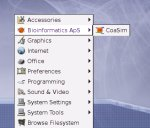
\includegraphics{figs/coasim-menu}
  \caption{The CoaSim icon in the menu.}
  \label{fig:menu}
\end{wrapfigure}

In future releases we plan to build more power into the GUI version,
but at this moment limited resources forces us to focus our efforts on
one of the versions, and therefore the GUI version is limited compared
to the Guile Scheme version.

Once CoaSim has been install, on most platforms it will appear in the
menu, as shown in Fig.~\ref{fig:menu}.  If it does not, however, it
can be started from the command line as
\begin{code}
> coasim_gui
\end{code}

Once started, the main window, shown on Fig.~\ref{fig:main}, appears.
This window is used to specify the markers to use in a simulation.
Using the tabs, different kinds of markers can be specified: trait
markers, used for specifying a trait of interest; SNP markers, similar
to trait markers, but with a different ascertainment bias; and
micro-satellite markers, with a different mutation model than the
other two.  Additional parameters for the simulation can be set in the
\emph{ARG Simulation Parameters} dialogue, shown in
Fig.~\ref{fig:arg-parameters}, opened from the \emph{Simulation} menu
in the main window.

\begin{figure}[tp]
  \centering
  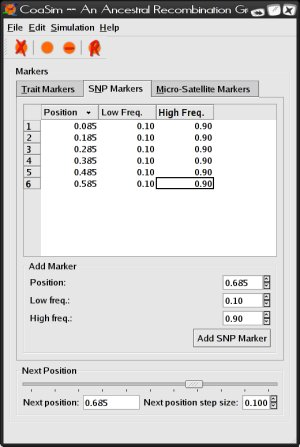
\includegraphics{figs/main-window}
  \caption{The CoaSim main window.  Used to set up markers for simulation.}
  \label{fig:main}
\end{figure}

\begin{figure}[tp]
  \centering
  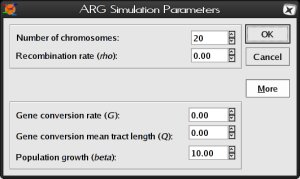
\includegraphics{figs/arg-parameters}
  \caption{Dialogue for setting ARG simulation parameters.}
  \label{fig:arg-parameters}
\end{figure}

Once the parameters have been set, the simulation can be started from
the \emph{Simulation} menu.  This opens the simulation monitor, shown
in Fig.~\ref{fig:monitor} and runs the simulation.  Once the
simulation has completed, the result is shown in the result dialogue
shown in Fig.~\ref{fig:results}.  From this dialogue it is possible to
save the result as a simple text file.

\begin{figure}[tp]
  \centering
  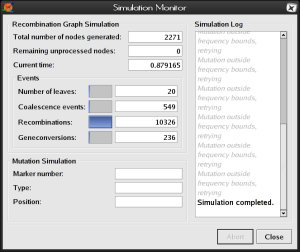
\includegraphics{figs/monitor}
  \caption{Simulation monitor, showing the progress of the monitor and
  different statistics about the simulation.}
  \label{fig:monitor}
\end{figure}

\begin{figure}[tp]
  \centering
  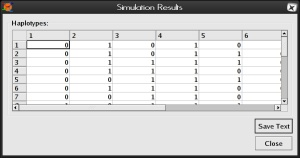
\includegraphics{figs/results}
  \caption{Simulation results.}
  \label{fig:results}
\end{figure}



\subsection{Using the Scheme-based CoaSim}
\label{sec:using-scheme-based}

Before using the guile-scheme based CoaSim \emph{it is necessary that
  you have installed the program}, not just compiled the program; at
least if you are using any of the scheme modules distributed with
CoaSim.  If the tool has not been properly installed, it will not be
able to locate the modules and the scripts, including several of the
included test scripts, will not be able to run.  If it is not possible
to install the modules globally, you can install the locally but you
will then need to set the \verb?GUILE_LOAD_PATH? environment variable
to let CoaSim know where the modules are installed.  Consult the Guile
manual for further details (\verb?http://www.gnu.org/software/guile/docs/?).

Once CoaSim is successfully installed, it can be run with any number
of files as argument:
\begin{code}
> coasim_guile file-1.scm file-2.scm ... file-n.scm
\end{code}
CoaSim will execute these files as scheme programs in turn,
remembering the state between them, a feature that is sometimes useful
for setting up a set parameters in one file, and then running
simulations in following files.  In most cases, though, a single file
will suffice for running one or more simulations.

Controlling the simulations through scheme makes CoaSim a very
flexible and powerful simulation tool. However, with flexibility
inevitably is associated some complexity, and while running simple
simulations through the scheme interface is quite simple, the more
complex simulation tasks requires a bit of knowledge about the Scheme
programming language and the scheme modules supplied with CoaSim.  To
keep this `getting started' guide short, we do not attempt to explain
the scheme interface to CoaSim in detail here---for this we refer to
the \emph{CoaSim Guile Manual}---instead we give a short introduction
to running very simple simulations, and give an overview of the
example scripts distributed with CoaSim.

A very simple use of CoaSim is to simulate coalescent trees.  A script
for that is shown here:
\begin{code}
(let* ((m (snp-marker 0.5 0 1))
       (arg (simulate (list m) 10))
       (tree (car (local-trees arg))))
  (display tree))
\end{code}
This might look a bit complicated, but if you break it down in the
three phases mentioned at the beginning of this section---setting up
parameters, running a simulation, and analysing the result---it is
really not.

The \verb?(let* ...)? construction is just a way of creating a block
of scheme code, that lets us define variables.  The variables we
define in the code above are \texttt{m}, \texttt{arg}, and
\texttt{tree}.  The variable \texttt{m} is part of the first phase,
setting up parameters.  In fact, it is the only part of this phase.
The expression
\begin{code}
(let* ((m (snp-marker 0.5 0 1))
       ...)
  )
\end{code}
defines \texttt{m} to be a SNP marker, positions at the middle of the
genomic region we consider (position 0.5), with the 0-allele frequency
to be between 0 and 1, i.e. unrestricted.

The next line is the simulation phase, it defines the variable
\texttt{arg} to hold the ARG that is the result of the simulation.
\begin{code}
(let* (...
       (arg (simulate (list m) 10))
       ...)
  )
\end{code}

The first parameter of the simulation is a list of markers---in this
case just the single marker \texttt{m} from above.  The second
argument is the number of chromosomes to simulate, in this case 10.

Once the ARG is simulated, we can start the analysis phase; in this
example it is very simple: we simply print the coalescent tree.  We
obtain the tree by taking the first local tree from the ARG
(recombinations will split the genomic region into intervals with
different trees, but in this example will only get a single tree, so
the tree we are interested in is the first and only local tree).
Selecting this tree is done with
\begin{code}
(let* (...
       (tree (car (local-trees arg))))
  )
\end{code}
where \texttt{local-trees} extracts the list of local trees from the
ARG, and \texttt{car} (which is scheme-speak for the head of a list)
selects the first tree in the list.  The final statement in the script:
\begin{code}
(let* (...)
  (display tree))
\end{code}
simply prints the tree.


As another simple application, consider simulating a list of SNP
sequences.  A script for simulating 100 sequences with 10 SNP markers
in each is shown here:
\begin{code}
(use-modules ((coasim rand)))
(let* ((markers (make-random-snp-markers 10 0 1))
       (seqs (simulate-sequences markers 10 :rho 400)))
  (display seqs)(newline))
\end{code}

The first line
\begin{code}
(use-modules ((coasim rand))
\end{code}
includes the \texttt{(coasim rand)} module, which is used for
generating random markers (markers on random positions, in this case).

The following lines are similar to the script above
\begin{code}
(let* ((markers (make-random-snp-markers 10 0 1))
       (seqs (simulate-sequences markers 10 :rho 400)))
  (display seqs)(newline))
\end{code}
except that we now make a list of 10 markers, using a function from
the module we just included, \texttt{make-random-snp-markers},
simulate a set of sequences rather than the ARG, and with 100 rather
than 10 chromosomes, and with the recombination rate $\rho$ set to 400
(which for an effective population size $N_e$ of 10,000 roughly
correspond to 1cM).  Actually, the \texttt{simulate-sequences}
function is just a short-cut for an ARG simulation using
\texttt{simulate}, as before, and a function, \texttt{sequences}, for
extracting the sequences from an ARG.  The following script is thus
equivalent to the script above:
\begin{code}
(let* ((markers (make-random-snp-markers 10 0 1))
       (arg (simulate markers 10 :rho 400))
       (seqs (sequences arg)))
  (display seqs)(newline))
\end{code}
A script very similar to the tree simulation script.

Printing sequences with the \texttt{display} function will print a
list of lists; this is a format that is very simple for Scheme to read
and manipulate, but is usually not suitable for other analysis tools.
To print the sequences in a more traditional form of a sequence per
line, with the sequences printed as space-separated numbers, we can
use the \texttt{(coasim io)} module like this:
\begin{code}
(use-modules ((coasim rand)) (coasim io))
(let* ((markers (make-random-snp-markers 10 0 1))
       (seqs (simulate-sequences markers 10 :rho 400)))
  (call-with-output-file "positions.txt" 
    (marker-positions-printer markers))
  (call-with-output-file "sequences.txt"     
    (sequences-printer seqs)))
\end{code}
Here, the positions are written to the file \texttt{positions.txt} and
the sequences to the file \texttt{sequences.txt}.  The
\texttt{call-with-output-file} function is a way of opening a file for
writing and the \texttt{marker-positions-printer} and
\texttt{sequences-printer} take care of writing the output.

Running several simulations is not much more complicated than running
a single simulation.  Consider the following script that simulates 10
coalescent trees instead of only one:
\begin{code}
(use-modules ((coasim batch) :select (repeat)))
(repeat 10 (let* ((m (snp-marker 0.5 0 1))
                  (arg (simulate (list m) 10))
                  (tree (car (local-trees arg))))
             (display tree)))
\end{code}

The first line loads a module---just as we loaded the module
\texttt{(coasim rand)} above---but with a slight variation that only
loads a single function, \texttt{repeat}, and not the entire module.
In most cases you would just load the module, but we only load
\texttt{repeat} here to give an example of how this is done.  Loading
single functions from a module, instead of the entire module, can be
useful to avoid name-clashing in your scripts.

The next statement calls \texttt{repeat} with two arguments, the
number of simulations to run, and the code for the simulation; the
later you will recognise as the same code we used above to simulate a
single tree.

When conducting a large number of simulations, it is usually not
desirable to print all results, but rather to calculate some
statistics about the simulations.  As a very simple example, instead
of printing simulated trees, we can calculate the mean of the total
branch length of the trees.  For this we again use the module
\texttt{(coasim batch)}, but rather than using \texttt{repeat} we use
the function \texttt{tabulate} that lets us collect simulation
results.  The complete script looks like this:
\begin{code}
(use-modules ((coasim batch) :select (tabulate)))
(let* ((no-iterations 10000)
       (branch-lengths
        (tabulate no-iterations
                  (let* ((m (snp-marker 0.5 0 1))
                         (arg (simulate (list m) 10))
                         (tree (car (local-trees arg))))
                    (total-branch-length tree)))))
  (display (/ (apply + branch-lengths) no-iterations))(newline))
\end{code}

We fix the number of simulations to use and give it the name
\texttt{no-iterations}, using the \texttt{(let* ...)} syntax, we then
call \texttt{tabulate} with the number of iterations and the code for
simulating a tree and getting its branch length.  The main difference
in the simulation code is that we call the function
\texttt{total-branch-length} on the tree instead of printing it using
\texttt{display}.

The result of the \texttt{tabulate} call is a list of simulation
results, which we store in the variable \texttt{branch-lengths}.  We
then use this list to calculate the mean by summing the values (using
the function call \texttt{(apply + branch-lengths)} and dividing it
with the number of iterations \texttt{(/ ... no-iterations)}, and we
finally print the result using \texttt{display}.


Calculating the branch-length like this is a bit silly, since we can
calculate the expected branch length for a coalescent tree with $n$
nodes simply as
\[
  2\sum_{i=1}^{n-1}\frac{1}{i}
\]
but when we add exponential growth, no such simple formula exists.  As
a final example of running simulations in CoaSim, consider calculating
the mean branch length for various growth parameters $\beta$:

\begin{code}
(use-modules ((coasim batch) :select (tabulate)))

(define betas '(0 10 20))
(define (mean-branch-length beta)
  (let* ((no-iterations 1000)
         (branch-lengths
          (tabulate no-iterations
            (let ((arg (simulate (list (snp-marker 0.5 0 1)) 10 :beta beta)))
              (total-branch-length (car (local-trees arg)))))))
    (/ (apply + branch-lengths) no-iterations)))

(display (map mean-branch-length betas))(newline)
\end{code}

This looks very similar to the simulation code above, but we have now
defined a list of $\beta$ values:
\begin{code}
(define betas '(0 10 20))
\end{code}
and made the mean branch lengths calculation into a function of $\beta$:
\begin{code}
(define (mean-branch-length beta)
    ...)
\end{code}

The way that $\beta$ is specified to the simulation is through the
keyword argument \texttt{:beta value} in
\begin{code}
    (simulate (list (snp-marker 0.5 0 1)) 10 :beta beta)
\end{code}

The final line in the script `maps' the \texttt{mean-branch-length}
function over the $\beta$ values, which means that it applies the
function on each $\beta$ and collect the results in a list, and it
then prints this list using \texttt{display}.

In all honesty, calculating the mean branch length in this way is a
bit inefficient, since we build a list of all simulated values and
then sum the elements; it would be more efficient to calculate the sum
during the iterations.  This can also be done, using the \texttt{fold}
function rather than \texttt{tabulate}:

\begin{code}
(use-modules ((coasim batch) :select (fold)))

(define betas '(0 10 20))
(define (mean-branch-length beta)
  (let* ((no-iterations 10)
         (branch-sum
          (fold no-iterations (lambda (val sum) (+ val sum)) 0
                (let* ((m (snp-marker 0.5 0 1))
                       (arg (simulate (list m) 10 :beta beta))
                       (tree (car (local-trees arg)))
                       (branch-length (total-branch-length tree)))
                  branch-length))))
    (/ branch-sum no-iterations)))

(display (map mean-branch-length betas))(newline)
\end{code}

The \texttt{fold} method, which will be familiar to people with
exposure to functional programming, builds a value from the
simulations using a function for combining the result so far with the
latest simulated value, and an initial value.  In the example above,
the function
\begin{code}
     (lambda (val sum) (+ val sum))
\end{code}
adds a new value to the sum so far, with the initial value 0.  Folding
with this pair of combination function and initial value lets us
calculate the sum of branch lengths without building a list of the
simulated values.


For further examples, see \verb?/usr/local/share/coasim/test-input/?
containing the files (in order of increasing complexity):
\begin{itemize}
\item \texttt{tree.scm}---the tree example from above.
\item \texttt{sequences.scm}---the sequence example from above.
\item \texttt{snp-haplotype.scm}---a more detailed example of
  simulating SNP sequences.
\item \texttt{snp-haplotype-split.scm}---an example of
  simulating SNP sequences and splitting them into cases and controls,
  based on a trait-marker.
\item \texttt{more-trees.scm}---the simulation and printing of several
  trees, from above.
\item \texttt{more-sequences.scm}---simulation of several sequences,
  writing them to different files.
\item \texttt{mean-branch-length.scm}---the calculation of the mean branch
  length of trees, from above.
\item \texttt{more-mean-branch-length.scm}---the calculation of the mean branch
  length of trees with various $\beta$ values, from above.
\item \texttt{fold-mean-branch-length.scm}---the calculation of the mean branch
  length of trees with various $\beta$ values using \texttt{fold}, as above.
\item \texttt{ms.scm}---an example of simulating sequences and
  outputting them in Hudson's ms format.
\end{itemize}

\end{document}

%% Local Variables: ***
%% TeX-command-default:"LaTeX PDF" ***
%% End: ***

% LocalWords:   CoaSim geneconversion haplotype haplotypes
